%&pdflatex
\documentclass[mathserif]{beamer}
\usetheme[progressbar=foot]{metropolis}
\setbeamertemplate{caption}[numbered]
\hypersetup{colorlinks, linkcolor=, urlcolor=blue}
\graphicspath{{pics/}}

\usepackage[utf8x]{inputenc}
\usepackage[T1]{fontenc}
\usepackage[english]{babel}

\usepackage{amssymb, amsmath, amsfonts, mathtools, mathrsfs}
\usepackage{subcaption} % for subfigures
\usepackage{comment}


%%% For multi-phase thermal fluid dynamics
\usepackage{physics}                        % for physics-oriented typesetting
\usepackage{siunitx}                        % for SI units

\newcommand{\bv}{\vb{u}}                    % velocity
\newcommand{\bn}{\vb{n}}                    % normal
\newcommand{\fusion}[1]{{#1}^\mathrm{fus}}  % fusion-related quantities
\newcommand{\xoverbrace}[2][\vphantom{\int}]{\overbrace{#1#2}}

%%% For the TikZ example
\newcommand{\bxi}{\boldsymbol{\xi}}
\newcommand{\LB}{\mathrm{LB}}
\newcommand{\DV}{\mathrm{DV}}

\usepackage{tikz}                           % for drawing
\usetikzlibrary{arrows, math, decorations.pathreplacing, calc}

\tikzset{
    >=latex',
    interface/.style={blue, very thick},
    ghost/.style={fill=gray!50},
    eqref/.style={red},
	mapping/.style={eqref, dashed},
    bolddot/.style={shape=circle, fill=black, scale=0.5},
}

\title{Introduction to \textrm{\LaTeX} and the related tools}
\author{Oleg Rogozin}
\institute{Skolkovo Institute of Science and Technology, Russia}
\date{}


\begin{document}

\frame{\titlepage}

\begin{frame}
  \frametitle{Plan}
  \begin{itemize}
      \item What is \textrm{\LaTeX}?
      \item Launch \href{https://overleaf.com}{OverLeaf} and study an example
      \item Short introduction in \textrm{\LaTeX} typesetting
      \item Questions \& Break
      \item Some examples of advanced \textrm{\LaTeX}
      \item Questions \& Break
      \item \href{https://www.lyx.org}{LyX} as a front end for \textrm{\LaTeX} by Prof.~Aslan Kasimov
      \item Formulation of the homework
  \end{itemize}
\end{frame}

\section{Introduction}

\begin{frame}
    \frametitle{Typesetting system}
    \centering
    \begin{columns}[T]
		\column{.5\textwidth}\centering\Large
		\textbf{Plain text \\[5pt] {\footnotesize (Separation of content \\[-10pt] and presentation)}} \\[10pt]
		\textrm{\LaTeX} \\ HTML \& CSS \\ Markdown \\ \dots \\[10pt]
		\footnotesize
		\begin{itemize}
		    \item focus on the content
		    \item best quality due to compilation
		    \item standard for scientific texts
		\end{itemize}

		\column{.6\textwidth}\centering\Large
		\textbf{Formatted text \\ (WYSIWYG)} \\[18pt]
		Microsoft Word \\ LibreOffice Writer \\ Apple Pages \\ \dots \\[10pt]
		\footnotesize
		\begin{itemize}
		    \item focus on the appearance
		    \item poor quality due to rendering on the fly
		    \item standard for bureaucratic reports
		\end{itemize}
	\end{columns}
\end{frame}

\begin{frame}
    \frametitle{}
    \centering
    Please, register in \href{https://overleaf.com}{OverLeaf}
    and create an example project.
    \pause

    Let's look through \href{https://www.overleaf.com/learn/latex/Learn_LaTeX_in_30_minutes}
    {OverLeaf quick-start guide} best suited for self-study.
\end{frame}

\section{Advanced examples}

\begin{frame}
    \frametitle{Multi-phase thermal fluid dynamics}\footnotesize
    The governing equations are as follows:
    \begin{gather*}
        \pdv{\alpha}{t} + \bv\vdot\grad\alpha = 0, \quad \pdv{\rho}{t} + \div(\rho\bv) = 0, \\
        \begin{aligned}
        \pdv{\rho\bv}{t} + \div(\rho\bv\bv) =
            &- \xoverbrace{\alert{K\alpha\frac{(1-\phi)^2}{\phi^3}\bv}}
                ^{\substack{\text{Darcy force with}\\\text{Kozeny--Carman}\\\text{permeability}}}
            + \xoverbrace{\div\vb*\tau}^\text{viscosity}
            - \xoverbrace{\grad{p}}^{\substack{\text{pressure}\\\text{force}}}\\
            &+ \xoverbrace{\gamma\kappa\grad\alpha}^{\substack{\text{surface}\\\text{tension}}}
            + \xoverbrace{\rho\vb{g}}^{\substack{\text{gravity}\\\text{force}}}
            + \xoverbrace{|\grad\alpha|\dv{\gamma}{T}\qty(\grad{T}
                - \bn\bn\vdot\grad{T})}^\text{Marangoni force},
        \end{aligned}\\
        \pdv{\rho h}{t} + \div(\rho h\bv)
            = \xoverbrace{\div(k\grad{T})}^\text{heat conduction}
            + \xoverbrace{\div(k\fusion{h}\grad{\phi})}^\text{fusion heat}
            + \xoverbrace{\div(\bv\vdot\vb*\tau)}^\text{viscous heat},
    \end{gather*}
    \scriptsize
    where \(\rho\) is the density, \(\bv\) is the velocity, \(T\) is the temperature,
    \(p\) is the pressure, \(\phi\) is the liquid fraction, \(\alpha\) is the gas fraction,
    \(K\) is the coefficient related to permeability of the mushy layer,
     \(\gamma\) is the coefficient of surface tension,
    \(\bn = \grad\alpha/|\grad\alpha|\) is the unit normal vector,
    \(\kappa = -\div{\bn}\) is the curvature, \(\vb{g}\) is the gravitational acceleration,
    \(k\) is the heat conductivity, \(\fusion{h}\) is the latent heat of fusion.
\end{frame}

\begin{frame}
    \frametitle{Drawing in \LaTeX{} by means of TikZ}
    \scriptsize\centering
    \begin{figure}
        \hspace{-20pt}
        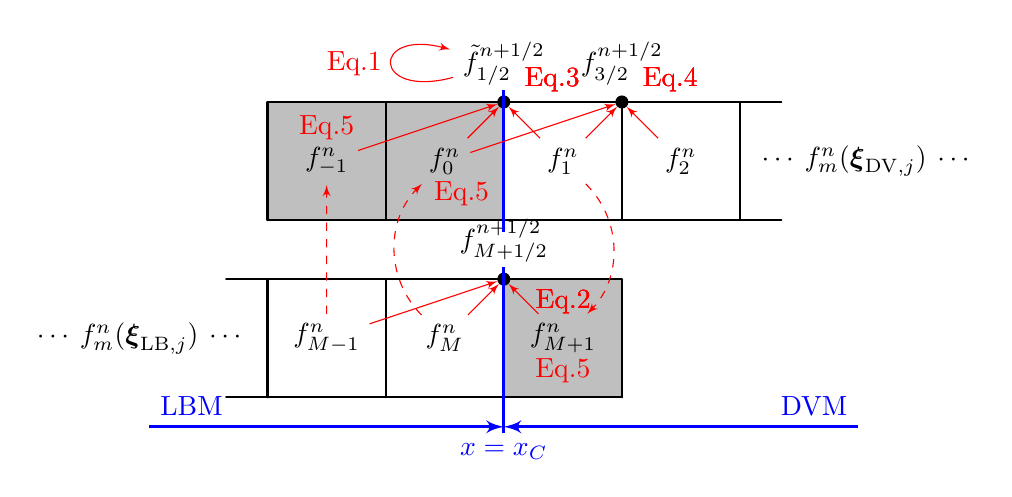
\begin{tikzpicture}[scale=0.75]
            \fill[ghost] (-4,2) -- (0,2) -- (0,0) -- (-4,0) -- cycle;
            \fill[ghost] (0,-1) -- (2,-1) -- (2,-3) -- (0,-3) -- cycle;
            \draw[thick, line cap=round, step=2] (-4,0) grid (4.7,2);
            \draw[thick, line cap=round, step=2, yshift=1cm] (-4.7,-4) grid (2,-2);
            \node[bolddot] (F_DV) at (0,2) {};
            \node[above] (F) at (F_DV.north) {$\tilde{f}^{n+1/2}_{1/2}$}
                edge [eqref, loop left] node {Eq.1} ();
            \node[bolddot, label=above:$f^{n+1/2}_{3/2}$] (F_DV3) at (2,2) {};
            \node[bolddot, label=above:$f^{n+1/2}_{M+1/2}$] (F_LB) at (0,-1) {};
            \node[left](f_LB-2) at (-4.2,-2) {$\cdots\:f^n_m(\bxi_{\LB,j})\:\cdots$};
            \node[right](f_DV3) at (4.2,1) {$\cdots\:f^n_m(\bxi_{\DV,j})\:\cdots$};
            \foreach \idx\i [evaluate={\x=2*\i-1}] in {M-1/-1,M/0,M+1/1} {
                \node (f_DV\i) at (\x,1) {$f^n_{\i}$};
                \node (f_LB\i) at (\x,-2) {$f^n_{\idx}$};
            };
            \node (f_DV2) at (3,1) {$f^n_2$};
            \draw[interface](0,2.2) -- (0,-0.2);
            \draw[interface](0,-.8) -- (0,-3.6) node[below] {$x=x_C$};
            \draw[->, interface] (-6,-3.5) node[above right] {LBM} -- (0,-3.5);
            \draw[<-, interface] (0,-3.5) -- (6,-3.5) node[above left] {DVM};
            \foreach \m in {LB,DV} \foreach \n in {f_\m-1,f_\m0,f_\m1} {
                \draw[->, eqref] (\n) -- (F_\m);
            }
            \foreach \m in {LB} \foreach \n in {f_\m-1,f_\m0,f_\m1} {
                \node at (F_\m) [eqref, below=8pt, right=8pt] {Eq.2};
            }
            \foreach \m in {DV} \foreach \n in {f_\m-1,f_\m0,f_\m1} {
                \node at (F_\m) [eqref, above=8pt, right=4pt] {Eq.3};
            }
            \foreach \m in {DV} \foreach \n in {f_\m0,f_\m1,f_\m2} {
                 \draw[->, eqref] (\n) -- (F_\m3);
                \node at (F_\m3) [eqref, above=8pt, right=4pt] {Eq.4};
            }
            \draw[->, mapping] (f_LB-1) -- (f_DV-1);
            \foreach \a/\b in {LB0/DV0,DV1/LB1}
                \draw[->, mapping] (f_\a) to[bend left=45] (f_\b);
            \foreach \n/\side/\offset in {f_DV-1/above/0,f_DV0.west/below right/1mm, f_LB1/below/0}
                \node at ($(\n) - (\offset,0)$) [eqref, \side=4pt] {Eq.5};
            \useasboundingbox (-4.2,-1.1) rectangle (2.2,2.8);
        \end{tikzpicture}
        \hspace{-20pt}
        \caption{\scriptsize
            The computational domain \(\Omega\) is divided into LB and DV subdomains,
            which are extended by the ghost cells (shown in gray).
            The vertical blue line highlight the coupling interface \(x=x_C\).
            The red arrows represent the dependency relations
            among the set of nodes in the extended \(\Omega\) for \(\xi_j>0\).
            The values in nodes pointed out by these arrows are calculated from the provided references.
            The dashed red arrows correspond to the projection of the solution onto the truncated Hermite basis.
        }
        \label{fig:coupling_scheme}
    \end{figure}
\end{frame}

\begin{frame}
    \frametitle{Bibliography utilities}
    \centering
    \begin{figure}
        \centering
        \begin{subfigure}[b]{0.3\textwidth}
            \includegraphics[width=\textwidth]{mendeley}
            \caption{Mendeley}
            \label{fig:gull}
        \end{subfigure}
        ~ %add desired spacing between images, e. g. ~, \quad, \qquad, \hfill etc.
          %(or a blank line to force the subfigure onto a new line)
        \begin{subfigure}[b]{0.3\textwidth}
            \includegraphics[width=\textwidth]{zotero}
            \caption{Zotero}
            \label{fig:tiger}
        \end{subfigure}
        ~ %add desired spacing between images, e. g. ~, \quad, \qquad, \hfill etc.
        %(or a blank line to force the subfigure onto a new line)
        \begin{subfigure}[b]{0.3\textwidth}
            \includegraphics[width=\textwidth]{jabref}
            \caption{JabRef}
            \label{fig:mouse}
        \end{subfigure}
    \end{figure}
\end{frame}

\begin{frame}
    \frametitle{Useful resources}
    General documentation:
    \begin{itemize}
        \item online: \href{https://en.wikibooks.org/wiki/LaTeX}{Wiki Books \LaTeX}
        \item offline (rus): \href{http://www.ccas.ru/voron/download/voron05latex.pdf}
            {K.~Vorontsov -- \LaTeX{} in Examples -- 2005}
    \end{itemize}
    Manuals for all packages:
    \begin{itemize}
        \item online: \href{https://ctan.org/}{Comprehensive \TeX{} Archive Network (CTAN)}
        \item offline: search PDF in your TeXLive distribution
    \end{itemize}
    Questions \& Answers:
    \begin{itemize}
        \item online: \href{https://tex.stackexchange.com/}{\LaTeX{} Stack Exchange}
    \end{itemize}
    \footnotesize
    P.S. Use \href{https://grammarly.com/}{Grammarly Premium} under Skoltech license
    to spellcheck your texts.
\end{frame}

\end{document}
